\documentclass[a4paper,12pt]{article}
\usepackage[margin=2cm]{geometry}

% Pacchetti utili di base
\usepackage[utf8]{inputenc}   % codifica dei caratteri
\usepackage[T1]{fontenc}      % font encoding
\usepackage{babel}
\babelprovide[import, main]{italian}
\usepackage{graphicx}         % immagini
\usepackage{hyperref}         % link cliccabili
\usepackage{amsmath}          % align center
\usepackage{amssymb}    % simboli matematici extra (\mathbb, \nabla, ecc.)
\usepackage{amsfonts}   % font matematici aggiuntivi
\usepackage{amsthm}     % se vuoi definire teoremi, definizioni, ecc.
\usepackage{float}       % per immagini non float
\usepackage{tikz}        % per barra sopra
\usepackage{mathcomp} % per simbolo siile al dollaro con due barre
\newcommand{\tripletilde}{\mathrel{\stackrel{\sim}{\stackrel{\sim}{\sim}}}}


% Informazioni sul documento
\title{Probabilità e statistica}
\author{Nicolò Giuliani}
\date{}


\begin{document}
\maketitle
\tableofcontents   % <-- genera automaticamente la pagina dell'indice
\newpage
\section{Spazi di probabilità}
Con \textit{probabilità} intendiamo la misura della certezza assoluta che un evento si verifichi o no. In matematica attribuiamo un valore compreso tra $[0,1]$ come intervallo tra il \textit{falso} e il \textit{vero}. 
\begin{itemize}
  \item $\mathbb{P} = 0$ significa che con certezza assoluta la proposizione è \textit{falsa}.
  \item $\mathbb{P} = 1$ significa che con certezza assoluta la proposizione è \textit{vera}.
  \item $\mathbb{P} \in {0,1}$ significa che la proposizione è probabile, più $\mathbb{P}(A)$ è vicina ad 1 più è più probabile che l'evento $A$ avvenga.
\end{itemize}
\textbf{Come calcoliamo la probabilità di un evento?} Abbiamo due modi di interpretazione
\begin{itemize}
  \item Approccio \textit{bayesano}: Si prendono tutte le informazioni che abbiamo a disposizione e arriviamo ad una assegnazione iniziale tramite generalmente simmetrie.
  \item Approccio \textit{frequentista}: Ripetiamo l'esperimento per ottenere un \textit{campione} di dati da analizzare tramite gli strumenti della statistica descrittiva.
  \begin{align*}
      \mathbb{P}(A) \approx \frac{n° \text{ volte che si verifica } A}{n}
  \end{align*}
\end{itemize}
Generalmente sono pochi i casi in cui si preferisce l'approccio bayesano perchè questo è molto difficile da applicare in problemi dove la simmetria non è ben definita o il problema non è ripetibile. Nella realtà gli esperimenti fisici possono essere ripetuti e l'approccio frequentista è la preferita. In ogni caso però le \textit{inferenze} (conclusioni) vanno validate con gli strumenti della statistica inferenziale.
\vspace{1em}\\
Possiamo riassumere che
\begin{itemize}
  \item Che cosè la probabilità? \textit{Filosofia}
  \item Come si stima la probabilità? \textit{Statistica}
  \item Quali assiomi verifica la probabilità? \textit{Matematica}
\end{itemize}
Per ora concentriamoci su quest'ultimo.
\subsection{Teoria degli insiemi}
Possiamo definire matematicamente un evento come un insieme. \\
Dato $\Omega$ un insieme e $\omega$ un suo elemento, quindi
\begin{align*}
    \omega \in \Omega \\
    \emptyset \in \Omega \\
    \Omega \in \Omega
\end{align*}
Definiamo \textbf{cardinalità} (numero di elementi) con
\begin{align*}
    | \Omega | \\
    \text{oppure} \\
    \# \Omega
\end{align*}
Definiamo \text{l'insieme delle parti} $\mathcal{P}(A)$ ovvero l'insieme di tutti i sottoinsiemi di $\Omega$ (insieme di insiemi).
\begin{align*}
  \Omega = \{1,2\} \\
  \mathcal{P}(\Omega) = \{\emptyset, \Omega, \{1\}, \{2\} \}
\end{align*}
e la sua cardinalità
\begin{align*}
  | \mathcal{P}(\Omega) | = 4
\end{align*}
\textbf{Operazioni insiemistiche} Ricordiamo unione, intersezione e complementazioni
\begin{align*}
A \cup B = \{\omega \in \Omega \, : \, \text{ $\omega$ appartiene ad almeno uno tra $A$ o $B$} \} \\
A \cap B = \{\omega \in \Omega \, : \, \text{ $\omega$ appartiene sia ad $A$ e $B$} \} \\
A^c = \{\omega \in \Omega \, : \, \text{ $\omega$ non appartiene ad $A$}\} \\
B \backslash A = \{\omega \in B \, : \, \text{$\omega$ non appartiene ad $A$} \}
\end{align*}
Ricordiamo anche le \textbf{leggi di De Morgan}:
\begin{itemize}
  \item per due insiemi 
  \begin{align*}
  (A \cup B)^c = A^c \cap B^c \\
  (A \cap B)^c = A^c \cup B^c
  \end{align*}
\end{itemize}
Ricordiamo le \textbf{proprietà distributive}
\begin{align*}
  A \cup ( B \cap C) = (A \cup B) \cap (A \cup C) \\
  A \cap (B \cup C) = (A \cap B) \cup (A \cap C)
\end{align*}
\textbf{Unioni e intersezioni infinite}
Si dice $A_1, \dots, A_n$ \textit{famiglia numerabile} o \textit{successione} di sottoinsiemi di $\Omega$, definiamo
\begin{align*}
  \bigcup_{n=1}^{\infty} A_n = \{\omega \in \Omega \, : \, \omega \in A \text{ per almeno un $n$}\} \\
  \bigcap_{n=1}^{\infty} A_n = \{\omega \in \Omega \, : \, \omega \in A \text{ per ogni un $n$}\}
\end{align*}
Anche per questo vengolo applicate le leggi di De Morgan.
\subsection{Modello matematico di un esperimento aleatorio}
Un \textbf{esperimento aleatorio} (fenomeno aleatorio/prova/situazione d'incertezza) è un esperimento che non conosciamo con certezza il risultato. Un \textbf{esito} è un suo ipotetio risultato. \\
Ora definiamo matematicamente: \\
\vspace{2px} \\
\fcolorbox{blue!75!black}{blue!5!white}{
\parbox{\linewidth}{
\textbf{Definizione}: Un \textbf{evento} è una affermazione riguardante l'ipotetico risultato dell'esperimento di cui possiamo dire con certezza se è vero o falso una volta noto l'esito del esperimento. Gli esisti per un evento vero si chiamano \textit{casi favorevoli} gli altri si chiamano casi contari.
}}
\vspace{2px} \\
Un evento lo definiamo con una lettera maiscola:
\begin{align*}
  A = \text{" esce un numero pari"}
\end{align*}
\vspace{2em} \\
Il \textbf{modello matematico} di un esperimento aleatorio è una descrizione sintetica dell'esperimento stesso attraverso la teoria degli insiemi.
\vspace{2px} \\
\fcolorbox{blue!75!black}{blue!5!white}{
\parbox{\linewidth}{
\textbf{Definizione}: Definiamo \textbf{spazio campionario} un insieme che contiene tutti gli ipotetici risultati dell'esperimento. Lo definiamo con $\Omega$. Un suo qualunque esito lo definiamo con $\omega$.
}}
\vspace{2px} \\
\fcolorbox{blue!75!black}{blue!5!white}{
\parbox{\linewidth}{
\textbf{Definizione}: Ogni evento (affermazione) è rappresentato da quel sottoinsieme di $\Omega$ che contiene i casi favorevoli (esiti per cui evento è sempre vero). Un qualunque sottoinsieme di $\Omega$ lo chiameremo ancora evento.
}}
\vspace{5px}\\
Quindi il termine evento indica sia il sottoinsieme che l'affermazione, utilizzeremo anche lo stesso simbolo (lettera maiscuola).
Alcuni eventi hanno nomi specifici:
\begin{itemize}
  \item \textit{Evento certo} è l'insieme $\Omega$, effermazione sempre vera qualunque sia l'esito.
  \item \textit{Evento impossibile} è l'insieme $\emptyset$, affermazione sempre falsa qualunque sia l'esito.
  \item \textit{Evento elementare} è un sottoinsieme di $\Omega$ che contiene un solo elemento, corrisponde ad un’affermazione che e' vera per un solo esito.
\end{itemize}
Come abbiamo visto gli eventi sono descritti sia da affermazioni che da insiemi. Sulle affermazioni possiamo eseguire le operazioni date dai \textit{connettivi logici} alle quali corrispondono alle relative \textit{operazioni insiemistiche}.
\[
\begin{array}{|c|c|}
\hline
\textsc{Connettivi logici} & \textsc{Operazioni/Relazioni insiemistiche} \\
\hline

\textbf{Disgiunzione} & \textbf{Unione} \\
A \ \text{o} \ B & A \cup B \\
\hline

\textbf{Congiunzione} & \textbf{Intersezione} \\
A \ \text{e} \ B & A \cap B \\
\hline

\textbf{Negazione} & \textbf{Complementazione} \\
\text{non } A & A^{c} \\
\hline

\textbf{Implicazione} & \textbf{Inclusione} \\
A \Rightarrow B & A \subset B \\
\hline

\textbf{Doppia implicazione} & \textbf{Uguaglianza} \\
A \Leftrightarrow B & A = B \\
\hline

\end{array}
\]
\subsection{Assiomi della probabilità}
\vspace{2px} 
\fcolorbox{blue!75!black}{blue!5!white}{
\parbox{\linewidth}{
\textbf{Assioma I}. A ciascun sottoinsieme (o evento) $A$ di $\Omega$ è assegnato un numero $\mathcal{P}(A)$ che verifica
\begin{align*}
  0 \leq \mathcal{P}(A) \leq 1
\end{align*}
Tale numero $\mathcal{P}(A)$ si chiama \textbf{probabilità} di $A$.
}}
\vspace{2px} \\
\fcolorbox{blue!75!black}{blue!5!white}{
\parbox{\linewidth}{
\textbf{Assioma II}. $\mathbb{P}(\Omega)=1$
}}
\vspace{2px} \\
\fcolorbox{blue!75!black}{blue!5!white}{
\parbox{\linewidth}{
\textbf{Assioma III}. Vale la proprietà di \textbf{additività numerabile}: Sia $A_1, A_2, \dots, A_n$ una successione di sottoinsiemi di $\Omega$ tra loro disgiunti e sia 
\begin{align*}
    A = \bigcup_{n=1}^{\infty} A_n
\end{align*}
Allora
\begin{align*}
    \mathbb{P}(A) = \bigcup_{n=1}^{\infty} \mathbb{P}(A_n) = \sum_{n=1}^{\infty} \mathbb{P}(A_n)
\end{align*}
}}
Quindi la probabilità $\mathbb{P}$ è una funzione una funzione che ad ogni sottoinsieme $A$ di $\Omega$ fa corrispondere un numero in $[0, 1]$:
\begin{align*}
  A \in \mathcal{P}(\Omega) \to \mathbb{P}(A) \in [0,1]
\end{align*}
dove $\mathcal{P}$ è l'insieme delle parti di $\Omega$ ed è il dominio, mentre il codominio è $[0,1]$:
\begin{align*}
    \mathbb{P} \, : \, \mathcal{P}(\Omega) \to [0,1]
\end{align*}
Una probabilità $\mathbb{P}$ si dice \textbf{discreta} se assume un numero finito di valori.\\
\vspace{2px} \\
\fcolorbox{blue!75!black}{blue!5!white}{
\parbox{\linewidth}{
\textbf{Definizione}:La coppia $(\Omega, \mathbb{P})$ si dice \textbf{spazio di probabilità} o modello matematico dell'esperimento aleatorio.
}}
\vspace{5px}\\
\subsection{Conseguenze degli assiomi}
\vspace{2px} 
\fcolorbox{blue!75!black}{blue!5!white}{
\parbox{\linewidth}{
\textbf{Teorema}: Sia $(\Omega, \mathbb{P})$ spazio di probabilità. Dagli assiomi I-II-III ricaviamo:
\begin{itemize}
  \item $\mathbb{P}(\emptyset)=0$
  \item \textbf{Addittività finita}: se $A$ e $B$ sono disgiunti allora
  \begin{align*}
      \mathbb{P}(A \cup B) = \mathbb{P}(A)+\mathbb{P}(B) - \mathbb{P}(A\cap B)
  \end{align*}
  \item $\mathbb{P}(A^c)=1-\mathbb{P}(A)$
  \item \textbf{Monotonia}: se $A \subset B$, allora $\mathbb{P}(A) \leq \mathbb{P}(B)$
\end{itemize}
}}
\vspace{5px}\\
Dimostrazione: 1 - Spazi di probabilità.pdf, pagina 12. \\
\vspace{2px} 
\fcolorbox{blue!75!black}{blue!5!white}{
\parbox{\linewidth}{
\textbf{Teorema}: Consideriamo un esperimento aleatorio descritto da uno spazio campionario finito
\begin{align*}
  \Omega = \{\omega_1, \dots, \omega_N\}
\end{align*}
con esiti equiprobabili
\begin{align*}
  \mathbb{P}(\{\omega_1\}) = \dots = \mathbb{P}(\{\omega_N\})
\end{align*}
In tal caso diciamo che $\mathbb{P}$ è la \textbf{probabilità uniforme} e valgono le seguenti proprietà:
\begin{itemize}
  \item dato un qualunque elemento elementare vale
  \begin{align*}
      \mathbb{P}(\{\omega_i\}) = \frac{1}{N}
  \end{align*}
  \item dato un qualunque evento $A$ vale la \textbf{formula di Laplace}
  \begin{align*}
      \mathbb{P}(A) = \frac{n° \text{ di eventi elementari che compongono $A$}}{N}  = \frac{| A |}{| \Omega |} = \frac{\textbf{casi favorelovi}}{\textbf{casi contrari}}
  \end{align*}
\end{itemize}
}}
\vspace{5px}\\
Dimostrazione: 1 - Spazi di probabilità.pdf, pagina 16. \\
Ora possiamo svolgere problemi di \hyperref[sec:calc_comb]{calcolo combinatorio!}\\
\vspace{2px} \\
\fcolorbox{blue!75!black}{blue!5!white}{
\parbox{\linewidth}{
\textbf{Teorema}: Formula dell’unione di due eventi, Siano $A$ e $B$ due eventi qualunque (non necessariamente disgiunti) allora
\begin{align*}
    \mathbb{P}(A \cup B) = \mathbb{P}(A) + \mathbb{P}(B) - \mathbb{P}(A \cap B)
\end{align*}
}}
\section{Probabilità codizionata e indipidenza}
Consideriamo l'evento $A$ e indichiama $\mathbb{P}(A)$ la sua probabilità. Veniamo a sapere con un altro evento $B$ avvenga, come calcoliamo la nuova probabilità che tenga conto?
\begin{align*}
  \mathbb{P}(A|B)
\end{align*}
La chiamiamo \textbf{probabilità condizionata} di $A$ dato $B$.\\
\vspace{2px} \\
\fcolorbox{blue!75!black}{blue!5!white}{
\parbox{\linewidth}{
\textbf{Definizione}: La probabilità condizionata di $A$ dato $B$ è
\begin{align*}
  \mathbb{P} = \frac{\mathbb{P}(A \cap B)}{\mathbb{P}(B)}
\end{align*}
}}
A parole possiamo dire
\begin{align*}
  \mathbb{P}(A|B) = \frac{\text{probabilità de casi veri favorevoli}}{\text{probabilità de casi veri possibili}}
\end{align*}
Non vale quasi mai l'uguaglianza 
\begin{align*}
  \mathbb{P}(A|B) \neq \mathbb{P}(B|A)
\end{align*}
Analizziamo ora dei casi un po particolari:
\begin{itemize}
  \item Caso $B = \Omega$:
  \begin{align*}
    \mathbb{P}(A| \Omega) = \frac{\mathbb{P}(A \cap \Omega)}{\mathbb{P}(\Omega)} = \mathbb{P}(A)
  \end{align*}
  \item Caso $A = \Omega$:
  \begin{align*}
      \mathbb{P}(\Omega|B) = \frac{\mathbb{P}(\Omega \cap B)}{\mathbb{P}(B)}= \frac{\mathbb{P}(B)}{\mathbb{P}(B)} = 1
  \end{align*}
  \item Caso $B \subset A$:
  \begin{align*}
      \mathbb{P}(A|B) = \frac{\mathbb{P}(A \cap B)}{\mathbb{P}(B)}= \frac{\mathbb{P}(B)}{\mathbb{P}(B)}=1 
  \end{align*}
\end{itemize}
\vspace{2px} 
\fcolorbox{blue!75!black}{blue!5!white}{
\parbox{\linewidth}{
\textbf{Teorema}: Sia $B$ un evento t.c. $\mathbb{P} > 0$. Allora valgono:
\begin{itemize}
  \item (Assioma I) Per ciascun evento (sottoinsieme) $A$ di $\Omega$, vale 
  \begin{align*}
    0 \leq \mathbb{P}(A|B) \leq 1
  \end{align*}
  \item $\mathbb{P}(\Omega | B) = 1$
  \item (Assioma III) Vale la proprietà di \textbf{addivitità numerabile}. Sia $A_1, \dots, A_{infty}$ successione di eventi disgiunti e sia
  \begin{align*}
    A = \bigcup_{n=1}^{\infty} A_n
  \end{align*}
  Allora vale
  \begin{align*}
    \mathbb{P}(A|B) = \sum_{n=1}^{\infty} \mathbb{P}(A_n | B)
  \end{align*}
  \item $\mathbb{P}(\emptyset | B) = 0$
  \item \textbf{addivitità finita}: se $A_1$ e $A_2$ sono disgiunti allora 
  \begin{align*}
      \mathbb{P}(A_1 \cup A_2 | B) = \mathbb{P}(A_1 | B) + \mathbb{P}(A_2 | B) 
  \end{align*}
  \item $\mathbb{P}(A^c | B) = 1 - \mathbb{P}(A | B)$
  \item \textbf{Monotonia}: se $A_1 \subset A_2$, allora 
  \begin{align*}
    \mathbb{P}(A_1 | B) \leq \mathbb{P}(A_2 | B)
  \end{align*}
\end{itemize}
}} 
\vspace{5px}\\
Dimostrazione: 2 - Probabilità condizionata e indipendenza.pdf, pagina 5. \\
Notiamo come la stessa probabilità condizionata sia anch'essa una probabilità
\begin{align*}
  \mathbb{P}(\cdot | B) \, : \, \mathcal{P}(\Omega) \to [0,1]
\end{align*}
\vspace{2em} \\
\subsection{Regola della catena}
Utilizzo della probabilità condizionata: \\
Alcune volte si utilizza la \textbf{regola della catena} (\textit{formula della probabilità composta})
\begin{align*}
  \mathbb{P}(A \cap B ) = \mathbb{P}(A | B)\mathbb{P}(B)
\end{align*}
con $\mathbb{P}(A | B)$ e $\mathbb{P}(A)$ noti.\\
\fcolorbox{blue!75!black}{blue!5!white}{
\parbox{\linewidth}{
\textbf{Teorema}: Siano $A$ e $B$ due eventi, $\mathbb{P}(B) > 0$. Vale la regola della catena:
\begin{align*}
  \mathbb{P}(A \cap B ) = \mathbb{P}(A | B)\mathbb{P}(B)
\end{align*}
In generale (con $\mathbb{P}(A_1 \cap \dots \cap A_{n-1}) > 0$
\begin{align*}
  \mathbb{P}(A_1 \cap \dots \cap A_n) = \mathbb{P}(A_n | A_1 \cap \dots \cap A_{n-1})\mathbb{P}(A_1)
\end{align*}
Da qui ricaviamo che 
\begin{align*}
  A_1 \cap \dots \cap A_{n-1} \subset A_1 \cap \dots \cap A_{n-2} \subset \dots \subset A_1
\end{align*}
}} \\
\vspace{5px}\\
Dimostrazione: 2 - Probabilità condizionata e indipendenza.pdf, pagina 6. \\
\vspace{2em} \\
\fcolorbox{blue!75!black}{blue!5!white}{
\parbox{\linewidth}{
\textbf{Definizione}: Si dice che $n$ eventi $B_1, \dots, B_n$ sono una \textbf{partizione} di $\Omega$ se:
\begin{itemize}
  \item $B_1, \dots, B_n$ sono disgiunti
  \item l'unione di $B_1, \dots, B_n$ è $\Omega$
  \begin{align*}
  \Omega = \bigcup_{i=1}^n B_n
\end{align*}
\end{itemize}
}} \\
\vspace{5px}\\
\subsection{Eventi indipendenti}
Un evento indipendente lo possiamo definire quando
\begin{align*}
  \mathbb{P}(A | B) = \mathbb{P}(A)
\end{align*}
Ovvero che la probabilità che si verifichi $A$ con o senza $B$ è la stessa.\\
\vspace{1px}\\
\fcolorbox{blue!75!black}{blue!5!white}{
\parbox{\linewidth}{
\textbf{Definizione}: Due eventi $A$ e $B$ si dicono \textbf{indipendenti} se
\begin{align*}
  \mathbb{P}(A \cap B) = \mathbb{P}(A)\mathbb{P}(B)
\end{align*}
}}
\\
\vspace{1px}\\
Scriveremo quindi 
\begin{align*}
  A \perp\!\!\!\perp B
\end{align*}
La proprietà di essere indipententi è ovviamente simmetrica.\\
\vspace{1px}\\
\fcolorbox{blue!75!black}{blue!5!white}{
\parbox{\linewidth}{
Vediamo la simmetria:
\begin{itemize}
  \item Se $\mathbb{P}(B) > 0$ allora 
  \begin{align*}
     A \perp\!\!\!\perp B \iff \mathbb{P}(A | B) = \mathbb{P}(A)
  \end{align*}
    \item Se $\mathbb{P}(A) > 0$ allora 
  \begin{align*}
     A \perp\!\!\!\perp B \iff \mathbb{P}(B | A) = \mathbb{P}(B)
  \end{align*}
\end{itemize}
Quindi se $\mathbb{P}(A) > 0$ e $\mathbb{P}(B) > 0$ allora le seguenti cose sono equivalenti:
\begin{align*}
  \mathbb{P}(A \cap B) = \mathbb{P}(A)\mathbb{P}(B), \quad \mathbb{P}(A | B) = \mathbb{P}, \quad \mathbb{P}(B | A) = \mathbb{P}(B)
\end{align*}
}}\\ 
\vspace{1px}\\
Dimostrazione: 2 - Probabilità condizionata e indipendenza.pdf, pagina 13. \\
\vspace{5px} \\
\fcolorbox{blue!75!black}{blue!5!white}{
\parbox{\linewidth}{
\textbf{Teorema}: Siano $A$ e $B$ due eventi indipententi. Allora anche $A^c$ e $B$ oppure $A$ e $B^c$ sono indipenti.
}}\\ 
\vspace{1px}\\
Dimostrazione: 2 - Probabilità condizionata e indipendenza.pdf, pagina 13. \\
\vspace{5px} \\
\fcolorbox{blue!75!black}{blue!5!white}{
\parbox{\linewidth}{
\textbf{Definizione}: Tre eventi $A,B,C$ si dicono \textbf{indipenti} se valgono simultaneamente:
\begin{align*}
  \mathbb{P}(A \cap B) = \mathbb{P}(A)\mathbb{P}(B)\\
  \mathbb{P}(A \cap C) = \mathbb{P}(A)\mathbb{P}(C)\\
  \mathbb{P}(B \cap C) = \mathbb{P}(B)\mathbb{P}(C)\\
  \mathbb{P}(A \cap B \cap C)=\mathbb{P}(A)\mathbb{P}(B)\mathbb{P}(C)
\end{align*}
}}\\ 
\vspace{1px}\\
\subsection{Formula delle probabilità totali}
\fcolorbox{blue!75!black}{blue!5!white}{
\parbox{\linewidth}{
\textbf{Teorema della formula delle probabilità totali}: Sia $B_1,\dots,B_n$ una partizione di $\Omega$ allora per ogni evento $A$ vale
\begin{align*}
  \underbrace{\mathbb{P}(A)}_\text{prob. totale di $A$} =\sum_{i=1}^n \underbrace{\mathbb{P}(A \cap B)}_\text{prob. parziale di $A$}
\end{align*}
Se inoltre si ha che $\mathbb{P}(B_i) > 0$ per ogni $i = 1,\dots,n$ allora vale
\begin{align*}
  \mathbb{P}(A) = \sum_{i=1}^n \mathbb{P}(A | B_i)\mathbb{P}(B_i)
\end{align*}
}}\\
\vspace{1px}\\
Dimostrazione: 2 - Probabilità condizionata e indipendenza.pdf, pagina 18.
\vspace{1px}\\
\subsection{Formula di Bayes}
\fcolorbox{blue!75!black}{blue!5!white}{
\parbox{\linewidth}{
\textbf{Teorema della formula di Bayes}: Siano $A$ e $B$ due eventi t.c. $\mathbb{P}(A) > 0, \, \mathbb{P}(B)>0$ allora vale
\begin{align*}
  \mathbb{P}(B | A) = \frac{\mathbb{P}(A|B)\mathbb{P}(B)}{\mathbb{P}(A)}
\end{align*}
}}\\
\vspace{1px}\\
Dimostrazione: 2 - Probabilità condizionata e indipendenza.pdf, pagina 21. \\
\vspace{1em}\\
Molto spesso la utilizziamo insieme alla formula delle probabilità totali:
\begin{align*}
  \mathbb{P}(B | A) = \frac{\mathbb{P}(A|B)\mathbb{P}(B)}{\mathbb{P}(A)} = \frac{\mathbb{P}(A|B)\mathbb{P}(B)}{\sum_{i=1}^n \mathbb{P}(A | B_i)\mathbb{P}(B_i)}
\end{align*}
\section{Calcolo combinatorio}
\label{sec:calc_comb}
Abbiamo detto che dato $\Omega$ finito ed esiti equiprobabili allora
\begin{align*}
  \Omega = \{\omega_1, dots, \omega_N\} \\
  \mathbb{P}(\{w_i\}) = \frac{1}{N}
\end{align*}
e che dato un qualsiasi evento $A$ vale la formula di Laplace
\begin{align*}
      \mathbb{P}(A) = \frac{n° \text{ di eventi elementari che compongono $A$}}{N}  = \frac{| A |}{| \Omega |} = \frac{\textbf{casi favorelovi}}{\textbf{casi contrari}}
\end{align*}
Studieremo ora il calcolo combinatorio che è lo strumento per svolgere questi calcoli anche quando tali numeri sono particolarmente elevati.\\
\subsection{Cardinalità e corrispondenza biunivoca}
Possiamo scrivere Laplace come 
\begin{align*}
  \mathbb{P} = \frac{| A |}{| \Omega |}
\end{align*}
\fcolorbox{blue!75!black}{blue!5!white}{
\parbox{\linewidth}{
\textbf{Definizione}: due insiemi $A$ e $B$ si dice $A$ \textit{è in corrispondenza biunivoca con} $B$ se esiste una funzione biettiva (iniettiva e suriettiva)
\begin{align*}
  f \, : \, A \to B
\end{align*}
ovvero 
\begin{align*}
  | A | = |B| \iff \text{$A$ e $B$ sono in corrispondenza biunivoca}
\end{align*}
}}\\
\vspace{1px}\\
\subsection{Fattoriale e coefficiente binomiale}
Ricordiamo che il \textit{coefficiente binomiale} è 
\begin{align*}
  \binom{n}{k} = \frac{n!}{k!(n-k)!} \text{ con $k \leq n$} \\
 = \binom{n}{n-k}
\end{align*}
e anche 
\begin{align*}
  \binom{n}{0}=\binom{n}{n}=1 \\
    \binom{n}{1}=1
\end{align*}
Per $k < n$ vale la formula di \textit{Stifel}
\begin{align*}
  \binom{n}{k} = \binom{n-1}{k-1}+\binom{n-1}{k}
\end{align*}
Infine vale anche la formula di \textit{Netwon} con $a,b  \in \mathbb{R}$
\begin{align*}
  (a+b)^n = \sum_{k=0}^n \binom{n}{k}a^kb^{n-k}
\end{align*}
\subsection{Metodo delle scelte successive}
Permette di determinare la cardinalità di un insieme una volta caratterizzati univocamente i suoi elementi tramite un numero finito di scelte successive.\\
\vspace{1px}\\
\fcolorbox{blue!75!black}{blue!5!white}{
\parbox{\linewidth}{
\textbf{Metodo delle scelte successive}: Supponiamo che \textbf{ciasun} elemento di un insieme $A$ possa essere determinato tramite \textbf{una e una sola} sequenza di $k$ scelte successive, in cui ogni scelta viene effettuata tra un numero fissato di possibilità (tale numero di possibilit`a, qui di seguito indicato con $n_1, \dots, n_k$ non dipende dalle scelte precedenti ma solo da $k$):
\begin{itemize}
  \item la prima scelta viene effettuata tra $n_1$ possibilità
  \item la seconda scelta viene effettuata tra $n_2$ possibilità
  \item $\dots$
  \item a $k$-esima scelta viene effettuata tra $n_k$ possibilità
\end{itemize}
Allora la cardinalità di $A$ è
\begin{align*}
  | A | = n_1 \cdot n_2 \cdot \dots \cdot n_k
\end{align*}
}}\\
\vspace{1px}\\
\subsection{Disposizioni e combinazioni}
\vspace{2px} 
\fcolorbox{blue!75!black}{blue!5!white}{
\parbox{\linewidth}{
\textbf{Definizione disposizioni con ripetizione}: Dato insieme $E$, $|E|=n$ e $k \in \mathbb{N}$. Indichiamo con $DK_{n,k}$, insieme delle disposizioni con $k$ elementi di $E$, ossia l'insieme di tutte le sequenze ordinate di $k$ di $E$ non necessariamente distinti
\begin{align*}
  & DR_{n,k} = \{(x_1,\dots,x_k) \, : \, x_i \in E\} = \underbrace{E \times \dots \times E}_\text{$k$ volte}\\
  & |DR_{n,k}| = n^k
\end{align*}
}}\\
\vspace{1px}\\
Possiamo notare come $DR_{n,k}$ esprime i modi in cui possiamo disporre in maniera ordinata e ripetuta un numero $k$ di oggetti scelti da un insieme di $n$ oggetti.\\
\vspace{1px}\\
\fcolorbox{blue!75!black}{blue!5!white}{
\parbox{\linewidth}{
\textbf{Definizione disposizioni semplici}: Dato $E$ insieme e $|E|=n$ e $k \leq n$. Indichiamo con $D_{n,k}$ l'insieme delle disposizioni semplici di $k$ elementi di $E$, ovvero l'insieme che comprende tutte le sequenze ordinate di $k$ elementi distinti di $E$
\begin{align*}
  & D_{n,k} = \{(x_1,\dots,x_k) \, : \, x_i \in E \text{ distinti}\}\\
  & |D_{n,k}| = n(n-1)\dots (n-k-1) = \frac{n!}{(n-k)!}
\end{align*}
}}\\
\vspace{1px}\\
Possiamo notare come $D_{n.k}$ esprime i modi in cui possiamo disporre, in maniera ordinata e non ripetuta, un numero $k$ di oggetti scelti da un insieme di $n$ oggetti.\\
\vspace{1px}\\
\fcolorbox{blue!75!black}{blue!5!white}{
\parbox{\linewidth}{
\textbf{Definizione permutazioni}: Sia $E$ insieme, $|E|=n$. Indichiamo con $P_n$ l'insieme delle permutazioni degli $n$ elementi di $E$, ossia l'insieme $D_{n,k}$
\begin{align*}
  |P_n| = |D_{n,k}| =  n!
\end{align*}
}}\\
\vspace{1px}\\
Possiamo notare come $P_n$ esprime i modi in cui possiamo disporre, in maniera ordinata e non ripetuta, $n$ oggetti.\\
\vspace{1px}\\
\fcolorbox{blue!75!black}{blue!5!white}{
\parbox{\linewidth}{
\textbf{Definizione combinazione}: Dato $E$ insieme, $|E|=n$ e $k \leq n$. Indichiamo con $C_{n,k}$ l'insieme delle combinazioni (semplici o senza ripetizioni) di $k$ elementidi $E$, ossia la famiglia dei sottoinsiemi di $E$ di cardinalità $k$
\begin{align*}
  & C_{n,k} = \{A \subset E: \, |A|=k \}\\
  & |C_{n,k}| = \binom{n}{k}
\end{align*}
}}\\
\vspace{1px}\\
Vale anche la seguente equivalenza
\begin{align*}
  & \frac{n!}{(n-k)!} = |C_{n,k}|k! \\
  & |D_{n,k}| = |C_{n,k}| |P_k|
\end{align*}
\begin{figure}[H]
    \centering
    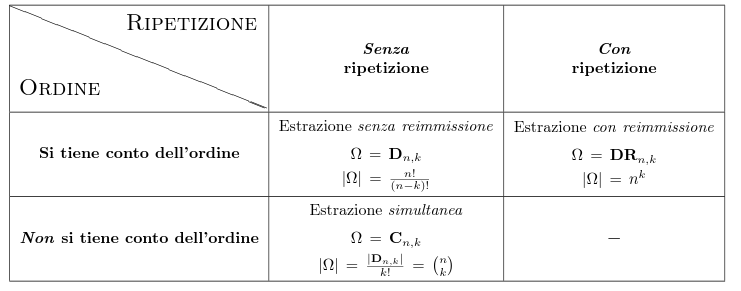
\includegraphics[width=0.8\textwidth]{img/rip.png}
\end{figure}
\begin{align*}
  \frac{\text{casi favorevoli in }C_{n,k}}{\text{casi possibili in }C_{n,k}} = \frac{k! (\text{casi favorevoli in }C_{n,k})}{k! (\text{casi possibili in }C_{n,k})} = \frac{\text{casi favorevoli in }D_{n,k}}{\text{casi possibili in }D_{n,k}}
\end{align*}
% Salvo il formato originale

% Forzo la numerazione
\addtocounter{section}{-1} % riporta il contatore a 3
\renewcommand{\thesection}{3.5}
\section{Variabili aleatorie}
\fcolorbox{blue!75!black}{blue!5!white}{
\parbox{\linewidth}{
\textbf{Definizione}: Un evento è una affermazione riguardante l’ipotetico risultato dell’esperimento aleatorio, di cui è possibile dire con certezza se è vera oppure falsa una volta noto l’esito dell’esperimento aleatorio.
}}\\
\vspace{1px}\\
\fcolorbox{blue!75!black}{blue!5!white}{
\parbox{\linewidth}{
\textbf{Definizione}: Ogni evento è rappresentato dal sottoinsieme di $\Omega$ costituito dai casi favorevoli. Un qualunque sottoinsieme di $\Omega$ lo chiamiamo ancora evento.
}}\\
\vspace{1px}\\
\fcolorbox{blue!75!black}{blue!5!white}{
\parbox{\linewidth}{
\textbf{Definizione}: Una \textbf{variabile aleatoria} è una affermazione riguardante l'ipotetico risultato dell'esperimento aleatorio. Tale affermazione identifica uno e un solo numero reale una volta noto l’esito dell’esperimento aleatorio.
}}\\
\vspace{1px}\\
In altre parole, mentre per un evento ha senso domandarsi "\textit{è vero oppure no?}", per una variabile aleatoria ha senso chiedersi "\textit{quanto vale?}".\\
Una variabile aleatoria viene indicata con una lettere maiscola.\\
\vspace{1px}\\
\fcolorbox{blue!75!black}{blue!5!white}{
\parbox{\linewidth}{
\textbf{Definizione}: Ogni variabile aleatoria è rappresentata dalla funzione $\Omega$ in $\mathbb{R}$ il cui valore numerico in corrispondenza di un qualunque esito dell’esperimento aleatorio, coincide con quanto fornito dall’affermazione.\\
Una qualunque funzione da $\Omega$ in $\mathbb{R}$ la chiameremo \textbf{variabili aleatoria}.
}}\\
\vspace{1px}\\
Il termine \textit{variabile aleatoria} indica sia l'affermazione che la funzione.
\subsection{Distribuzione di una variabile aleatoria}
\fcolorbox{blue!75!black}{blue!5!white}{
\parbox{\linewidth}{
\textbf{Definizione}: Sia $(\Omega, \mathbb{P})$ uno spazio di probabilità e $X \, : \, \Omega \to \mathbb{R}$ una variabile aleatoria. Si dice che $E \subset \Omega$ è un evento associato ad $X$ se esiste un sottoinsiene di $B$ dell'insieme dei numeri reali $\mathbb{R}$ t.c.
\begin{align*}
 & E = \{\omega \in \Omega: \, X(\omega) \in B\}\\
 & = "\text{sottoinsiemedi $\Omega$ costituito da tutti e soli gli esiti $\omega$ per cui $X(\omega) \in B$}".\\
\end{align*}
Viceversa, dato un qualunque $B \subset \mathbb{R}$ il sottoinsieme di $\Omega$ dato da
\begin{align*}
  \{\omega \in \Omega: \, X(\omega) \in B\}
\end{align*}
si chiama \textbf{evento associato ad} $X$.\\
Per brevità indicheremo il sottoinsieme
\begin{align*}
  \{\omega \in \Omega: \, X(\omega) \in B\}
\end{align*}
nel modo seguente
\begin{align*}
  \{X \in B\} \text{ oppure } (X \in B)
\end{align*}
}}\\
\vspace{1px}\\
Ad ogni variabile aleatoria $X$ è associato un oggetto di fondamentale importanza, la distribuzione o legge di $X$, che verrà indicata con $\mathbb{P}_X$ . Essa è una probabilità su $\mathbb{R}$.\\
\fcolorbox{blue!75!black}{blue!5!white}{
\parbox{\linewidth}{
\textbf{Definizione}: Sia $(\Omega, \mathbb{P})$ uno spazio di probabilità e $X \, : \, \Omega \to \mathbb{R}$ una variabile aleatoria. Si chiama \textbf{distribuzione} di $X$ la probalità
\begin{align*}
  \mathbb{P}_X \, : \, \mathcal{P}(\mathbb{R}) \to [0,1]
\end{align*}
definita da 
\begin{align*}
  \mathbb{P}_X(B) = \mathbb{P}(X \in B), \quad \forall B \subset \mathbb{R}
\end{align*}
Per dire che $X$ ha distribuzione $\mathbb{P}_X$ scriveremo
\begin{align*}
  X \sim \mathbb{P}_X
\end{align*}
}}\\
\vspace{1px}
\paragraph{Variabili aleatorie costanti de delta di Dirac} Sia $X$ la variabile aleatoria costante da 
\begin{align*}
  X(\omega) = a, \quad \forall \omega \in \Omega
\end{align*}
dove $a$ è un numero reale fissato. Possiamo calcolare esplicitamente la distribuzione di $X$ per ogni $B \subset \mathbb{R}$
\begin{align*}
  \mathbb{P}_X(B) = \mathbb{P}(X \in B) = \begin{cases}
    \mathbb{P}(\Omega), \text{ se $a \in B$}\\
    \mathbb{P}(\emptyset), \text{ se $a \notin B$}
  \end{cases} = \begin{cases}
    1, \text{ se $a \in B$}\\
    0, \text{ se $a \notin B$}
  \end{cases}
\end{align*}
Notiamo che $\mathbb{P}_X$ coincide con $\delta_a$ (delta di Dirac in $a$).\\
\paragraph{Variabili aleatorie indicatrici} Siano $A$ un evento e $X=1_A$, la variabile aleatoria indicatrice relativa all'evento $A$. Anche in questo caso possiamo calcolare in maniera esplicita la distribuzione di $X$. Infatti per ogni $B \subset \mathbb{R}$
\begin{align*}
  \{X \in B\} = \begin{cases}
    A, \text{ se $1 \in B$ e $0 \notin B$}\\
    A^c \text{ se $1 \notin B$ e $0 \in B$}\\
    \Omega, \text{ se $1 \notin B$ e $0 \in B$}\\
    \emptyset, \text{ $se 1 \in B$ e $0 \notin B$}
  \end{cases}
\end{align*}
Quindi
\begin{align*}
  \mathbb{P}_X(B) = \begin{cases}
     \mathbb{P}(A), \text{ se $1 \in B$ e $0 \notin B$}\\
    1 - \mathbb{P}(A)\text{ se $1 \notin B$ e $0 \in B$}\\
    1, \text{ se $1 \notin B$ e $0 \in B$}\\
    0, \text{ se $1 \in B$ e $0 \notin B$}
  \end{cases}
\end{align*}
In altri termini si ha che $\mathbb{P}_X$ coincide con la seguente combinazione convessa di $\delta_0$ e $\delta_1$: $(1-\mathbb{P}(A))\delta_0 + \mathbb{P}(A)\delta_1$. Quindi
\begin{align*}
    X \sim (1-\mathbb{P}(A))\delta_0 + \mathbb{P}(A)\delta_1
\end{align*}
Infatti per ogni $B \subset \mathbb{R}$
\begin{align*}
  (1-\mathbb{P}(A))\delta_0 + \mathbb{P}(A)\delta_1 = \begin{cases}
     \mathbb{P}(A), \text{ se $1 \in B$ e $0 \notin B$}\\
    1 - \mathbb{P}(A)\text{ se $1 \notin B$ e $0 \in B$}\\
    1, \text{ se $1 \notin B$ e $0 \in B$}\\
    0, \text{ se $1 \in B$ e $0 \notin B$}
  \end{cases}
\end{align*}
Questo dimostra che $\mathbb{P}_X = (1-\mathbb{P}(A))\delta_0 + \mathbb{P}(A)\delta_1 $. Tale probabilità si chiama \textit{distribuzione di Bernoulli di parametro $\mathbb{P}(A)$}.
\subsection{Funzione di ripartizione (CDF)}
\fcolorbox{blue!75!black}{blue!5!white}{
\parbox{\linewidth}{
\textbf{Definizione}: Sia $(\Omega, \mathbb{P})$ uno spazio di probabilità aleatoria. Si chiama \textbf{funzione di ripartizione CDF} di $X$ la funzione
\begin{align*}
  F_X \, : \, \mathbb{R} \to [0,1]
\end{align*}
definita da 
\begin{align*}
  F_X(x) = \mathbb{P}(X \leq x) = \mathbb{P}_X((-\infty,x]), \quad \forall x \in \mathbb{R}
\end{align*}
Per dire che $X$ ha funzione di ripartizione $F_X$ scriveremo
\begin{align*}
  X \sim F_X
\end{align*}
}}\\
\vspace{1px}\\
\paragraph{Variabili aleatorie costanti} Sia $a$ un numero reale e $X$ la variabile alleatoria costante e uguale ad $a$. Allora
\begin{align*}
  F_X(x) = \begin{cases}
    0, \text{ se $x < a$}\\
    1, \text{ se $x \geq a$}
  \end{cases}  
\end{align*}
\paragraph{Variabili aleatorie indicatrici} Sia $A$ un evento e $X=1_A$. Allora
\begin{align*}
  F_X(x) = \begin{cases}
    0,  &x < 0\\
    1-\mathbb{P}(A), &0 \leq x < 1\\
    1, &x \geq 1
  \end{cases}
\end{align*}
\fcolorbox{blue!75!black}{blue!5!white}{
\parbox{\linewidth}{
\textbf{Teorema}: Sia $(\Omega, \mathbb{R})$ uno spazio di probabilità e $X \, : \, \Omega \to \mathbb{R}$ una variabile aleatoria. La funzione di ripartizione $F_X$ di $X$ verifica le seguenti proprietà:
\begin{itemize}
  \item $F_X$ è monotona crescente (non necessariamente strettamente)
  \item $F_X$ è continua a destra: $\lim_{y \to x+} F_X(X) \quad \forall x \in \mathbb{R}$
  \item $\lim_{x \to - \infty} F_X(x)=0$
  \item $\lim_{x \to +\infty} F_X(x)=1$
\end{itemize}
Viceversa se la funzione $G : \mathbb{R} \to [0,1]$ verifica tutte le proprietà, allora esistono uno spazio di probabilità $(\Omega, \mathbb{P})$ ed una variabile aleatoria $X$ t.c. $G=F_X$.
}}\\
\vspace{1px}\\
Dimostrazione: 3.5 - Variabili aleatorie.pdf, pagina 12.\\
\vspace{1px}\\
\fcolorbox{blue!75!black}{blue!5!white}{
\parbox{\linewidth}{
\textbf{Lemma}: Sia $(\Omega, \mathbb{P})$ uno spazio di probabilità. Allora $\mathbb{P}$ verifica le seguenti proprità di stabilità per i limiti monotoni:
\begin{itemize}
  \item siano $(A_n)_n$ una successione di eventi con $A_n \subset A_{n+1}$ e $A = \bigcup_n A_n$, allora vale che 
  \begin{align*}
      \lim_{n\to + \infty}\mathbb{P}(A_n) = \mathbb{P}(A)
  \end{align*}
  \item siano $(A_n)_n$ una successione di eventi con $A_n \supset A_{n+1}$ e $A = \bigcap_n A_n$, allora vale che 
  \begin{align*}
      \lim_{n\to + \infty}\mathbb{P}(A_n) = \mathbb{P}(A)
  \end{align*}
\end{itemize}
}}\\
\vspace{1px}\\
Dimostrazione: 3.5 - Variabili aleatorie.pdf, pagina 11.\\
\vspace{1px}\\
\fcolorbox{blue!75!black}{blue!5!white}{
\parbox{\linewidth}{
\textbf{Teorema probabilità di intervalli in termini di $F_X$}: Valgono le seguenti uguaglianze
\begin{align*}
\mathbb{P}(X = x) &= F_X(x) - F_X(x-) \\
\mathbb{P}(x < X \leq y) &= F_X(y) - F_X(x) \\
\mathbb{P}(x \leq X \leq y) &= F_X(y) - F_X(x-) \\
\mathbb{P}(x \leq X < y) &= F_X(y-) - F_X(x-) \\
\mathbb{P}(x < X < y) &= F_X(y-) - F_X(x)
\end{align*}
}}\\
% Ripristino formato normale
\renewcommand{\thesection}{\arabic{section}}
\setcounter{section}{3} % importante!
\section{Variabili aleatorie discrete}
La \textit{non definizione} dice: una variabile aleatoria si dice \textbf{discreta} se assume un numero finito (o al pi`u un’infinit`a numerabile) di valori.\\
\fcolorbox{blue!75!black}{blue!5!white}{
\parbox{\linewidth}{
\textbf{Definizione}: Sia $(\Omega, \mathbb{P})$ uno spazio di probabilità e $X$ una variabile aleatoria. La funzione $P_X \, : \, \mathbb{R} \to [0,1]$ data da 
\begin{align*}
  p_X(x) = \mathbb{P}(X=x), \quad \forall x \in \mathbb{R}
\end{align*}
si chiama \textbf{densità discreta} o \textbf{funzione di massa di probabilità} (PMF) di $X$.
}}
\vspace{2px} \\
Si noti che $p_X(x)$ è la probabilità che la variabile aleatoria $X$ assuma il valore $x$. Per tale ragione, $p_X (x)$ verifica necessariamente le disuguaglianze:
\begin{align*}
  0 \leq p_X(x) \leq 1, \quad \forall x \in \mathbb{R}
\end{align*}
La definizione di variabile aleatoria discreta fa intervenire la funzione $p_X$.\\
\fcolorbox{blue!75!black}{blue!5!white}{
\parbox{\linewidth}{
\textbf{Definizione}: Sia $(\Omega, \mathbb{P})$ uno spazio di probabilità e $X$ una variabile aleatoria. Si dice che $X$ è una \textbf{variabile aleatoria discreta} (in breve v.a.d.) se esiste un sottoinsieme $\mathcal{S}_X$ di $\mathbb{R}$, finito o al più infinito numerabile, quindi
\begin{align*}
  \mathcal{S}_X = \{x_1,\dots, x_n\} \text{ oppure } \mathcal{S}_X = \{x_1, \dots, x_i, \dots\}
\end{align*}
tale che:
\begin{itemize}
  \item $p_X(x_i) > 0 \forall x_i \in \mathcal{S}$ (\textit{minimalità} di $\mathcal{S}_X$) 
  \item $\mathbb{P}(X \in \mathcal{S}_X) = \sum_i p_X(x_i)=1$
\end{itemize}
L'insieme $\mathcal{S}_X$ si chiama \textbf{supporto} di $X$.
}}
\vspace{2px} \\
\paragraph{Tabella della densità discreta} Nel caso in cui $\mathcal{S}_X$ sia un insieme finito, quindi $\mathcal{S}_X = \{x_1,\dots,x_n\}$
\begin{align*}
  \begin{array}{c|c|c|c|c}
  X & x_1 & x_2 & \cdots & x_n \\
  \hline
  p_X & p_X(x_1) & p_X(x_2) & \cdots & p_X(x_n)
  \end{array}
\end{align*}
\paragraph{Variabili aleatorie costanti} Sia $a$ un numero reale e $X$ la variabile aleatoria costante uguale ad $a$. Allora $X$ è una variabile aleatoria discreta con supporto $\mathcal{S}_X = \{a\}$ e densità discreta.
\begin{align*}
  \begin{array}{c|c}
  X & a \\
  \hline
  p_X & 1
  \end{array}
\end{align*}
\paragraph{Variabili aleatorie indicatrici} Sia $A$ un evento e $X = 1_A$ la variabile aleatoria indicatrice relativa all’evento $A$. Allora $X$ è una variabile aleatoria discreta con supporto $\mathcal{S}_X = \{0, 1\}$ e densità discreta
\begin{align*}
  \begin{array}{c|c|c}
  X & 0 & 1 \\
  \hline
  p_X & 1-\mathbb{P}(A) & \mathbb{P}(A)
  \end{array}
\end{align*}
\subsection{Caratterizzazione delle variabili aleatorie discrete}
\fcolorbox{blue!75!black}{blue!5!white}{
\parbox{\linewidth}{
\textbf{Teorema}: Sia $(\Omega, \mathbb{P})$ uno spazio di probabilità e $X$ una variabile aleatoria. Le seguenti affermazioni sono equivalenti:
\begin{itemize}
  \item $X$ è una variabile aleatoria discreta
  \item $F_X$ è una funzione costante a tratti
  \begin{align*}
      & F_X(x_i)-F_X(x_i-)=p_X(x_i)\\
      & F_X(x) = \sum_{x_i \leq x} p_X (x_i) \quad \forall x \in \mathbb{R}
  \end{align*}
  \item $\mathbb{P}_X$ la distribuzione di $X$ è concentrata nei punti $x_1, x_2, \dots$ di $\mathcal{S}_X$
  \begin{align*}
      \mathbb{P}_X = \sum_i p_X(x_i) \delta_{x_i}
  \end{align*}
  Infine vale la formula
  \begin{align*}
    \mathbb{P}(X \in B) = \sum_{x_i \in B} p_X (x_i) \quad \forall B \subset \mathbb{R}
  \end{align*}
\end{itemize}
}}
\subsection{Indici di sintesi di una distribuzione: $\mu$ e $\sigma^2$}
La distribuzione o legge di una variabile aleatoria puo' essere descritta in maniera sintetica tramite due quantita' numeriche, la \textbf{media} (o valore atteso) e la varianza.\\
La media e' un indice di posizione, ovvero indica qual e' il valore “centrale” della distribuzione.
\begin{align*}
  \mu_\text{artim} = \frac{x_1+\dots+x_n}{n}
\end{align*}
Questa e' una \textit{media pesata}, ovvero tutti gli $x_i$ hanno lo stesso peso $\frac{1}{n}$.\\
La \textbf{varianza} e' un indice di dispersione, ossia dice quanto la distribuzione si concentra attorno alla media.
\begin{align*}
  & \frac{(x_1-\mu)^2 + \dots + (x_n-\mu)^2}{n} \\
  & = \frac{1}{n}\| x - \mu1 \|^2
\end{align*}
\subsubsection{Media o valore atteso}
\fcolorbox{blue!75!black}{blue!5!white}{
\parbox{\linewidth}{
  \textbf{Definizione}: Sia $x$ una variabile aleatoria discreta con supporto $\mathcal{S}_X = \{x_1, x_2, \dots\}$. La media (o valore atteso) di $X$ e' data da:
  \begin{align*}
    \mathbb{E}[X] = \sum_i x_i p_X(x_i)
  \end{align*}
  La media la indichiamo con $\mu$ oppure $\mu_X$.\\ 
  Il simbolo $\mathbb{E}$ significa \textit{expected value} (valore atteso).
}}\\
\vspace{5px}\\
\fcolorbox{blue!75!black}{blue!5!white}{
\parbox{\linewidth}{
  \textbf{Teorema}: Sia $X$ una variabile aleatoria discreta con densita' $p_X$ e supporto $\mathcal{S}_X=\{x_1,x_2,\dots\}$. Inoltre siano $h \, : \, \mathbb{R}\to\mathbb{R}$ e $Y = h(X)$. Allora
  \begin{align*}
    \mathbb{E}[Y] = \mathbb{E}[h(X)] = \sum_i h(x_i)p_X(x_i)
  \end{align*}
}}\\
\vspace{5px}\\
\fcolorbox{blue!75!black}{blue!5!white}{
\parbox{\linewidth}{
\textbf{Teorema Linearita' del valore atteso}: Sia $X$ una variabile aleatoria discreta. Inoltre siano $h \, : \, \mathbb{R}\to\mathbb{R}$, $g \, : \, \mathbb{R}\to\mathbb{R}$ e $a,b \in \mathbb{R}$ costanti. Allora
\begin{align*}
  \mathbb{E}[aX+b] = a\mathbb{E}[X]+b
\end{align*}
In generale:
\begin{align*}
  \mathbb{E}[a h(X)+ b g(X)] = a \mathbb{E}[h(X)]+b \mathbb{E}[g(X)]
\end{align*}
}}\\
\subsubsection{Varianza}
\fcolorbox{blue!75!black}{blue!5!white}{
\parbox{\linewidth}{
\textbf{Definizione}: Sia $X$ una variabile aleatoria discreta con densita' discreta $p_X$ e supporto $\mathcal{S}_X=\{x_1, x_2, \dots\}$. La varianza di $X$ e' data da:
\begin{align*}
  \text{Var}(X) = \mathbb{E}[(X - \mathbb{E}[X])^2] = \sum_i (x_i - \mathbb{E}[X])^2 p_X(x_i)
\end{align*}
La varianza si indica con $\sigma^2$ oppure $\sigma_X^2$.\\
La radice quadrata della varianza si chiama \textbf{deviazione standard} (o scarto quadratico medio o anche scostamento quadratico medio) e si indica con $\sigma$ oppure $\sigma_X$.
}}\\
\vspace{5px}\\
\fcolorbox{blue!75!black}{blue!5!white}{
\parbox{\linewidth}{
\textbf{Teorema}: Sia $X$ una variabile aleatoria discreta con densita' discretsa $p_X$ e supporto $\mathcal{S}_X = \{x_1, x_2, \dots\}$. Vale che 
\begin{align*}
  \text{Var}(X) = \mathbb{E}[X^2]-\mathbb{E}[X]^2 = \sum_i x_i^2 p_X(x_i)-\mathbb{E}[X]^2
\end{align*}
}}\\
\vspace{5px}\\
\fcolorbox{blue!75!black}{blue!5!white}{
\parbox{\linewidth}{
\textbf{Teorema  Proprieta' della varianza}: Siano $X$ una variabile aleatoria discreta e $a,b \in \mathbb{R}$ costanti. Allora
\begin{itemize}
  \item $\text{Var}(X)>\geq 0$
  \item $\text{Var}(b) = 0$ e viceversa: se $\text{Var}(X)=0$ allora $X$ e' una variabile aleatoria costante
  \item $\text{Var}(aX+b) = a^2 \text{Var}(X)$
\end{itemize} 
}}\\
\subsection{Distribuzioni discrete notevoli}
In questa sezione vediamo le principali distribuzioni discrete.
\vspace{1em}\\
\paragraph{Distribuzione uniforme discreta} Sia $\{x_1, \dots, x_n\}$ un sottoinsieme finito di $\mathbb{R}$. Diciano che $X$ ha distribuzione uniforme discreta sull'insieme $\{x_1, \dots, x_n\}$ se $X$ e' una variabile aleatoria discreta con $\mathcal{S}_X = \{x_1, \dots, x_n\}$ e densita' discreta data da
\[
\begin{array}{c|c|c|c|c}
X & x_1 & x_2 & \dots & x_n \\
p_X & \frac{1}{n} & \frac{1}{n} & \dots & \frac{1}{n}
\end{array}
\]
In tal caso scriviamo
\begin{align*}
  X \sim \text{Unif}(\{x_1, \dots, x_n\})
\end{align*}
Si noti che 
\begin{align*}
  \mathbb{E}[X] = \mu_\text{aritm} = \frac{x_1 + \dots + x_n}{n}\\
  \text{Var}(X) = \frac{(x_1 - \mathbb{E}[X])^2 + \dots + (x_1 - \mathbb{E}[X])^2}{n}
\end{align*}
\paragraph{Distribuzione di Bernoulli} Sia $0 \leq p \leq 1$. Diciamo che $X$ ha \textbf{distribuzione di Bernoulli} (o bernoulliana) di parametro $p$ se $X$ e' una variabile aleatoria discreta con $\mathcal{S}_X=\{0,1\}$ e densita' discreta data da
\begin{align*}
  \begin{array}{c|c|c}
  X & 0 & 1 \\
  \hline
  p_X & 1-p & p
  \end{array}
\end{align*}
In tal caso scriveremo
\begin{align*}
  X \sim B(p)
\end{align*}
Le variabili aleatorie di Bernoulli sono tutte e sole variabili aleatorie indicatrici. Infatti:
\begin{align*}
  X = 1_A, \quad \text{con } A =\{X = 1\}
\end{align*}
Si noti che 
\begin{align*}
  \mathbb{E}[X] = p\\
  \text{Var}(X) = p(1-p)
\end{align*}
\paragraph{Distribuzione binomiale} Consideriamo ora una generalizzazione della distribuzione bernoulliana: la \textit{distribuzione binomiale}. \\
Immaginiamo ora di ripetere $n$ volte l'esperimento aleatorio a cui l'evento $A$ si riferisce, in modo tale che i vari esperimenti siano tra loro “indipendenti”. Per ciascun esperimento consideriamo la corrispondente v.a. bernoulliana. Abbiamo dunque $n$ variabili aleatorie bernoulliane:
\begin{align*}
  X_1 \sim B(p), \quad X_2 \sim B(p), \quad \dots, \quad X_n \sim B(p)
\end{align*}
Consideriamo la seguente variabile aleatoria
\begin{align*}
  X = "\text{n. di successi negli $n$ esperimenti}"
\end{align*}
dove "\textit{successo}" si intende che l'evento $A$ si sia verificato.\\
Quindi $X$ e' il numero di volte che $A$ si e' verificato negli $n$ esperimenti. Notiamo che:
\begin{align*}
  X = X_1 + \dots + X_n
\end{align*}
\vspace{5px}\\
\fcolorbox{blue!75!black}{blue!5!white}{
\parbox{\linewidth}{
\textbf{Proposizione}: Siano $0 \leq p \leq 1, n \in \mathbb{N}$ e $X \sim B(n,p)$. Allora
\begin{align*}
  \mathbb{E}[X] = np\\
  \text{Var}(X) = np(1-p)
\end{align*}
}}\\
\vspace{5px}\\
\paragraph{Distribuzione di Poisson} La distribuzione di Poisson che ora introduciamo e' un “caso limite” della distribuzione binomiale, che si ottiene a partire dalla distribuzione binomiale quando
\begin{align*}
  n \to + \infty, \quad p \to 0, \quad np \to \lambda
\end{align*}
dove $\lambda > 0$ e' un costante fissata.\\
Anche se in modo impreciso, possiamo dire piu' semplicemente che se $X \sim B(n, p)$, $n$ e' “molto grande” e $p$ e' “molto piccolo”, allora $X$ ha approssimativamente distribuzione di Poisson di parametro $\lambda = np$.\\
Diciamo che $X$ ha distribuzione di Poisson di parametro $\lambda$ se $X$ e' un variabile aleatoria discreta con $\mathcal{S}_X = \{0,1,2,\dots\}$ e densita' discreta data da
\begin{align*}
  p_X(k) = \mathbb{P}(X=k) = e^{-\lambda}\frac{\lambda^k}{k!} \quad \forall k = 0,1,2,\dots
\end{align*}
In tal caso scriviamo 
\begin{align*}
  X \sim \text{Poisson}(\lambda)
\end{align*}
Si ricprdi che 
\begin{align*}
  \sum_{k=0}^{+\infty}\frac{x^k}{k!}=e^x
\end{align*}
Quindi si verifica che
\begin{align*}
  \sum_{k=0}^{+\infty} p_X(k) = \sum_{k=0}^{+\infty}\frac{x^k}{k!} = 1
\end{align*}
\vspace{5px}\\
\fcolorbox{blue!75!black}{blue!5!white}{
\parbox{\linewidth}{
  \textbf{Proposizione} Siano $\lambda > 0$ e $X \sim \text{Poisson}(\lambda)$. Allora
  \begin{align*}
    \mathbb{E}[X] = \lambda \\
    \text{Var}(X) = \lambda
  \end{align*}
}}
\section{Variabili aleatorie continue}
Se dobbiamo definire per esempio la vita di un componente $X$ diremo che la sua vita' e' maggiore uguale ad zero, ovvero $\mathcal{S}_X = \{0, + \infty\}$.\\
Innanzitutto, poiche' $X$ puo' assumere un’infinit`a continua di valori, l’eventualit`a che ne assuma esattamente uno in particolare (ad esempio il numero $x = 3,45362$) e' praticamente impossibile.
\begin{align*}
  p_X(x) = \mathbb{P}(X=x)=0 \quad \forall x \in \mathbb{R} \\
  \mathbb{P}(a \leq X \leq b) > 0 \quad \text{ se } [a,b] \subset [0, +\infty]
\end{align*}
In altri termini, la densita' discreta $p_X$ per una variabile aleatoria continua e' sempre identicamente uguale a zero, non gioca dunque alcun ruolo.
\subsection{Definizioni di densita' continua e v.a. continua}
\fcolorbox{blue!75!black}{blue!5!white}{
\parbox{\linewidth}{
\textbf{Definizione}: Una funzione $f : \mathbb{R} \to \mathbb{R}$ si dice \textbf{densita'} (continua) o \textbf{funzione di probabilita'} (PDF) se:
\begin{itemize}
  \item $f(x) \geq 0 \quad \forall x \in \mathbb{R}$
  \item $\int_{-\infty}^{+\infty} f(x) dx = 1$
\end{itemize}
}}\\
\vspace{1px}\\
\fcolorbox{blue!75!black}{blue!5!white}{
\parbox{\linewidth}{
\textbf{Definizione} Sia $(\Omega, \mathbb{P})$ uno spazio di probabilita' e $X$ una variabili aleatoria. Si dice che $X$ e' una variabile aleatoria continua (v.a.c) se esiste una densita' continua indicatacon $f_X$ t.c:
\begin{align*}
  \mathbb{P}(a \leq X \leq b) = \int_{a}^{b} f_X(x)dx, \quad \forall [a,b] \subset \mathbb{R} \\
  \mathbb{P}(X \in B) = \int_{B} f_X(x)dx, \quad \forall B \subset \mathbb{R}
\end{align*}
}}\\
Notiamo in particolare che la probabilita' che una variabile aleatoria continua $X$ assuma valori in un intervallo non dipende dal fatto che gli estremi dell’intervallo siano inclusi o esclusi, contrariamente a quanto accade per le variabile aleatorie discrete.\\
\vspace{1px}\\
\fcolorbox{blue!75!black}{blue!5!white}{
\parbox{\linewidth}{
\textbf{Teorema} Sia $X$ variabile aleatoria continua con densita' $f_X$
\begin{itemize}
  \item La densita' discreta di $X$ e' identicamente uguale ad zero
  \begin{align*}
    p_X(x) = 0 \quad \forall x \in \mathbb{R}
  \end{align*}
  \item La funziona di ripartizione di $X$ e' data da 
  \begin{align*}
    F_X(x) = \int_{-\infty}^{x} f_X (y)dy \quad \forall x \in \mathbb{R}
  \end{align*}
\end{itemize}
}}\\
\vspace{1px}\\
Possiamo dunque riassumere nel seguente schema le differenze principali tra variabili aleatorie discrete e continue:
\begin{figure}[H]
    \centering
    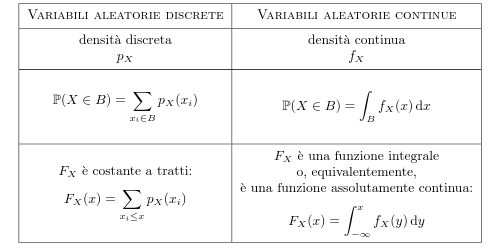
\includegraphics[width=0.8\textwidth]{img/tabella.png}
\end{figure}
\subsubsection{Dalla funzione di ripartizione alla densit`a continua}
\fcolorbox{blue!75!black}{blue!5!white}{
\parbox{\linewidth}{
\textbf{Proposizione} Sia $X$ una variabile aleatoria e indichiamo con $F_X$ la sua funzione di ripartizione. Supponiamo di sapere gia' che $X$ e' una variabile aleatoria continua (quindi sappiamo gia' che $F_X$ e' una funzione integrale). Allora, una densita' $f_X$ e' data da
\begin{align*}
  f_x(x) \, := \, F_X'(x)\quad \forall x \text{ in cui $F_X$ e' derivabile}
\end{align*}
mentre, nei punti in cui $F_X$ non e' derivabile, $f_X$ pue' essere definita in modo arbitrario.
}}\\
\vspace{1px}\\
\subsubsection{Funzioni di variabili aleatorie continue}
Siano $h : \mathbb{R} \to \mathbb{R}$ una qualunque funzione e $X$ una variabile aleatoria continua. Poniamo
\begin{align*}
  Y = h(X)
\end{align*}
Ricordiamo che quando $X$ e' discreta, $Y$ e' necessariamente anch’essa una variabile aleatoria discreta. Al contrario, quando $X$ e' continua, non possiamo dire nulla su $Y$. In particolare, $Y$ potrebbe essere discreta, continua, mista.\\
\vspace{5px}\\
La situazione pie' semplice si ha quando la variabile aleatoria $Y$ e' discreta. Si e' in tale
situazione quando $Y$ assume un numero finito o al pie' infinito numerabile di valori. Ad
esempio, se $h(x) = 1_{x>10}$ allora:
\begin{align*}
  Y = 1_{X > 10} = \begin{cases}
    1, \text{ se $X$ > 10}\\
    0, \text{ se $X \geq 10$}
  \end{cases}
\end{align*}
In tal caso $Y$ e' discreta in quanto assume solo due valori: $0$ e $1$. In particolare, $Y$ ha distribuzione di Bernoulli di parametro $p = \mathbb{P}(X > 10)$
\begin{align*}
  Y \sim B_(p)
\end{align*}
\subsection{Indici di sintesi di una distribuzione: $\mu$ e $\sigma^2$}
Come per le variabili aleatorie discrete, definiamo valore atteso e varianza per variabili aleatorie continue.
\subsubsection{Media o valore atteso}
\fcolorbox{blue!75!black}{blue!5!white}{
\parbox{\linewidth}{
\textbf{Definizione}: Sia $X$ una variabile aleatoria continua. La \textbf{media} (o valore atteso) di $X$ e' data da
\begin{align*}
  \mathbb{E}[X] = \int_{-\infty}^{+\infty} x f_X(x)dx
\end{align*}
La media si indicia anche con $\mu$ oppure $\mu_X$.
}}\\
\vspace{1px}\\
Capitera' spesso di dover calcolare il valore atteso di una funzione di $X$:
\begin{align*}
  Y = h(X)
\end{align*}
\fcolorbox{blue!75!black}{blue!5!white}{
\parbox{\linewidth}{
\textbf{Teorema}: Sia $X$ una variabile aleatoria continua. Inoltre, siano $h : \mathbb{R} \to \mathbb{R}$ e $Y = h(x)$. Allora:
\begin{align*}
  \mathbb{E}[Y] = \mathbb{E}[h(X)] = \int_{-\infty}^{+\infty} h(x)f_X(x)dx
\end{align*}
}}\\
Ricordiamo infine la propriet`a di linearit`a del valore atteso, gia' dimostrata nel caso discreto:\\
\vspace{5px}\\
\fcolorbox{blue!75!black}{blue!5!white}{
\parbox{\linewidth}{
\textbf{Teorema Linearita' del valore atteso}: Sia $X$ una variabile aleatoria discreta. Inoltre siano $h \, : \, \mathbb{R}\to\mathbb{R}$, $g \, : \, \mathbb{R}\to\mathbb{R}$ e $a,b \in \mathbb{R}$ costanti. Allora
\begin{align*}
  \mathbb{E}[aX+b] = a\mathbb{E}[X]+b
\end{align*}
In generale:
\begin{align*}
  \mathbb{E}[a h(X)+ b g(X)] = a \mathbb{E}[h(X)]+b \mathbb{E}[g(X)]
\end{align*}
}}\\
\subsubsection{Varianza}
\fcolorbox{blue!75!black}{blue!5!white}{
\parbox{\linewidth}{
\textbf{Definizione}: Sia $X$ una variabile aleatoria continua. La varianza di $X$ e' data da
\begin{align*}
  \text{Var}(X) = \mathbb{E}[(X-\mathbb{E}[X])^2] = \int_{-\infty}^{+\infty}(x-\mathbb{E}[X])^2 f_X(x)dx
\end{align*}
La varianza si indica anche con $\sigma^2$ oppure $\sigma_X^2$.\\
La radice quadrata della varianza si chiama deviazione standard (o scarto quadratico medio o anche scostamento quadratico medio) e si indica con $\sigma$ oppure $\sigma_X$.
}}\\
\vspace{1px}\\
\fcolorbox{blue!75!black}{blue!5!white}{
\parbox{\linewidth}{
\textbf{Teorema}: Sia $X$ una variabile aleatoria continua. Vale che
\begin{align*}
  \text{Var}(X) = \mathbb{E}[X^2]-\mathbb{E}[X]^2 = \int_{-\infty}^{+\infty} x^2 f_X(x)dx - \mathbb{E}[X]^2
\end{align*}
}}
\vspace{1px}\\
Ricordiamo infine le seguenti proprieta', gia' dimostrate nel caso discreto:\\
\fcolorbox{blue!75!black}{blue!5!white}{
\parbox{\linewidth}{
\textbf{Teorema  Proprieta' della varianza}: Siano $X$ una variabile aleatoria discreta e $a,b \in \mathbb{R}$ costanti. Allora
\begin{itemize}
  \item $\text{Var}(X)> 0$
  \item $\text{Var}(b) = 0$ e viceversa: se $\text{Var}(X)=0$ allora $X$ e' una variabile aleatoria costante
  \item $\text{Var}(aX+b) = a^2 \text{Var}(X)$
\end{itemize} 
}}\\
\subsection{Distribuzioni continue notevoli}
\paragraph{Distribuzione uniforme (continua)} Diciamo che $X$ ha \textbf{distribuzione uniforme (continua) su} $(a,b)$ se $X$ e' una variabile aleatoria continua con densita'
\begin{align*}
  f_X(x) = \begin{cases}
    \frac{1}{b-a}, \quad a < x < b\\
    0, \quad \text{ altrimenti}
  \end{cases}
\end{align*}
In tal caso scriveremo
\begin{align*}
  X \sim \text{Unif}(a,b)
\end{align*}
Si noti che 
\begin{align*}
  F_X(x) = \begin{cases}
    0, \quad x \leq a\\
    \frac{x-a}{b-a}, \quad a \leq x \leq b\\
    1, \quad x \geq b
  \end{cases}
\end{align*}
Inoltre
\begin{align*}
  & \mathbb{E}[X] = \int_{a}^b \frac{x}{b-a} dx = \frac{a+b}{2},\\
  & \text{Var}(X) = \mathbb{E}[X^2]- \mathbb{E}[X]^2 = \int_a^b \frac{x^2}{b-a} dx - (\frac{a+b}{2})^2 = \frac{(b-a)^2}{12}
\end{align*}
\paragraph{Distribuzione esponenziale} Sia $\lambda > 0$. Diciamo che $X$ ha \textbf{distribuzione esponenziale di parametro} $\lambda$ se $X$ e' una variabile aleatoria continua di densita'
\begin{align*}
  f_X(x) = \begin{cases}
    0, \quad x < 0\\
    \lambda e^{-\lambda x}, \quad x\geq 0
  \end{cases}
\end{align*}
In tal caso scriveremo
\begin{align*}
  X \sim \text{Exp}(\lambda)
\end{align*}
Si noti che 
\begin{align*}
  F_X(x) = \begin{cases}
    0, \quad x \leq 0\\
    1-e^{-\lambda x}, \quad x \geq 0
  \end{cases}
\end{align*}
Inoltre
\begin{align*}
  & \mathbb{E}[X] = \int_0^{+\infty} x \lambda e^{-\lambda x} dx = \frac{1}{\lambda}\\
  & \text{Var}(X) = \mathbb{E}[X^2] - \mathbb{E}[X]^2 = \int_{0}^{+\infty} x^2 \lambda e^{-\lambda x} dx - \frac{1}{\lambda^2} = \frac{1}{\lambda^2}
\end{align*}
La distribuzione esponenziale si usa ad esempio per descrivere il tempo di vita di un macchinario oppure di un componente. 
\paragraph{Distribuzione normale (o gaussiana)} Siano $\mu \in \mathbb{R}$ e $\sigma > 0$. Diciamo che $X$ ha una \textbf{distribuzione normale (o gaussiana) di mesia $\mu$ e varianza $\sigma^2$} se $X$ e' una variabile aleatoria continua con densita'
\begin{align*}
  f_X (x) = \frac{1}{\sigma \sqrt{2 \pi}} e^{- \frac{1}{2\frac{(x-\mu)^2}{\sigma^2}}, \quad \forall x \in \mathbb{R}}
\end{align*}
In tal caso scriviamo
\begin{align*}
  X \sim \mathcal{N}(\mu, \sigma^2)
\end{align*}
Diciamo inoltre che $X$ ha \textbf{distribuzione normale standard} se 
\begin{align*}
  X \sim \mathcal{N}(0,1)
\end{align*}
ovvero $X$ ha distribuzione normale di media $\mu=0$ e varianza $\sigma^2 = 1$. In tal caso la densita' di $X$ e' data da 
\begin{align*}
  f_X (x) = \frac{1}{\sqrt{2\pi}}e^{-\frac{1}{2}x^2}, \quad \forall x\in \mathbb{R}
\end{align*}
\fcolorbox{blue!75!black}{blue!5!white}{
\parbox{\linewidth}{
\textbf{Lemma (Intregrale di Gauss)}: Vale che
\begin{align*}
  \int_{-\infty}^{+\infty} e^{-x^2} dx = \sqrt(\pi)
\end{align*}
}}\\
\vspace{1px}\\
Di conseguenza avremo che 
\begin{align*}
  &   f_X (x) = \frac{1}{\sqrt{2\pi}}e^{-\frac{1}{2}x^2}, \quad \forall x\in \mathbb{R}\\
  & \int_{-\infty}^{+\infty} f_X (x) dx = 1
\end{align*}
\vspace{1px}\\
\fcolorbox{blue!75!black}{blue!5!white}{
\parbox{\linewidth}{
\textbf{Proposizione}: Siano $\mu \in \mathbb{R}, \sigma > 0$ e $X \in \mathcal{N}(\mu, \sigma^2)$
\begin{itemize}
  \item $\mathbb{E}[X] = \mu$
  \item $\text{Var}(X) = \sigma^2$
\end{itemize}
}}\\
\vspace{1px}\\
La distribuzione normale standard ha un ruolo fondamentale nello studio della distribu-
zione normale. Cio' deriva dal fatto che qualunque variabile aleatoria normale diventa, ese-
guendo un riscalamento e una traslazione (in una parola, \textit{standardizzando}), una variabile
aleatoria normale standard.\\
\fcolorbox{blue!75!black}{blue!5!white}{
\parbox{\linewidth}{
\textbf{Proposizione (Standardizzazione)} Siano $\mu \in \mathbb{R}, \sigma > 0$ e $X \in \mathcal{N}(\mu, \sigma^2)$. Allora
\begin{align*}
  Z = \frac{X - \mu}{\sigma}
\end{align*}
}}\\
\vspace{1px}\\
\fcolorbox{blue!75!black}{blue!5!white}{
\parbox{\linewidth}{
\textbf{Proposizione (Proprieta di $\Phi$)} Sia
\begin{align*}
  \Phi (x) = \int_{-\infty}^{x} \frac{1}{\sqrt{2 \pi}} e^{-\frac{1}{2} y^2} dy, \quad \forall x\in \mathbb{R}
\end{align*}
La funzione di ripartizione di una variabile aleatoria normale standard. $\Phi$ verifica le seguenti proprieta'
\begin{itemize}
  \item $\Phi(0) = \frac{1}{2}$
  \item $\Phi(-x) = 1 - \Phi(x), \quad \forall x \geq 0$
\end{itemize}
}}\\
\vspace{1px}\\
\section{Vettori aleatori}
test2
\end{document} 
